\section{引言}
\label{sec:intro}

基于 LLM 的代理~\cite{achiam2023gpt4,openclaw,opencode,claudecode,openai-codex-cli,wang2024agentsurvey} 正在重塑软件任务的完成方式。
开发者不再需要手工编写代码，而只需描述目标，
代理便会推理、调用工具并交付结果~\cite{yao2023react,qin2023toolllm}。
为支持这一范式，一个不断扩大的\emph{技能}生态~\cite{claude-agent-skills,anthropic-skills-repo,openclaw-medical-skills,skillssh} 已经出现，
旨在让代理执行更加可靠、实用。
技能主要由自然语言描述和脚本构成，其中封装了特定领域的
流程与最佳实践~\cite{anthropic-skills-blog}。
目前已有超过 100,000 个技能分布于主要平台~\cite{clawhub, skillssh}，
覆盖数据分析、金融、办公自动化、编程等众多领域。

然而，当前代理对技能的支持十分简单：系统把技能视为
附加上下文并直接传给模型。不同模型在理解和执行技能方面
存在显著差异~\cite{lu2024agentbench, han2026swe, li2026skillsbench}。
在横跨不同规模的八个模型中，
启用技能后，总体有 15\% 的任务性能下降（例如 Opus 4.6 为 7\%，Qwen3-30B 为 25\%）。
另有 17\% 的任务分数保持不变（不计完成率为 100\% 的任务），
并且在多达 87\% 的任务上，至少有一个模型使用技能后没有取得提升。
近期工作~\cite{han2026swe} 得出了相近结论：在 SWE-Benchmark 上，49 个技能中有 39 个未带来分数提升，另有 3 个造成明显的分数下降。

\begin{figure}[t]
  \centering
  \setlength{\abovecaptionskip}{5pt}
  \setlength{\belowcaptionskip}{-10pt}
  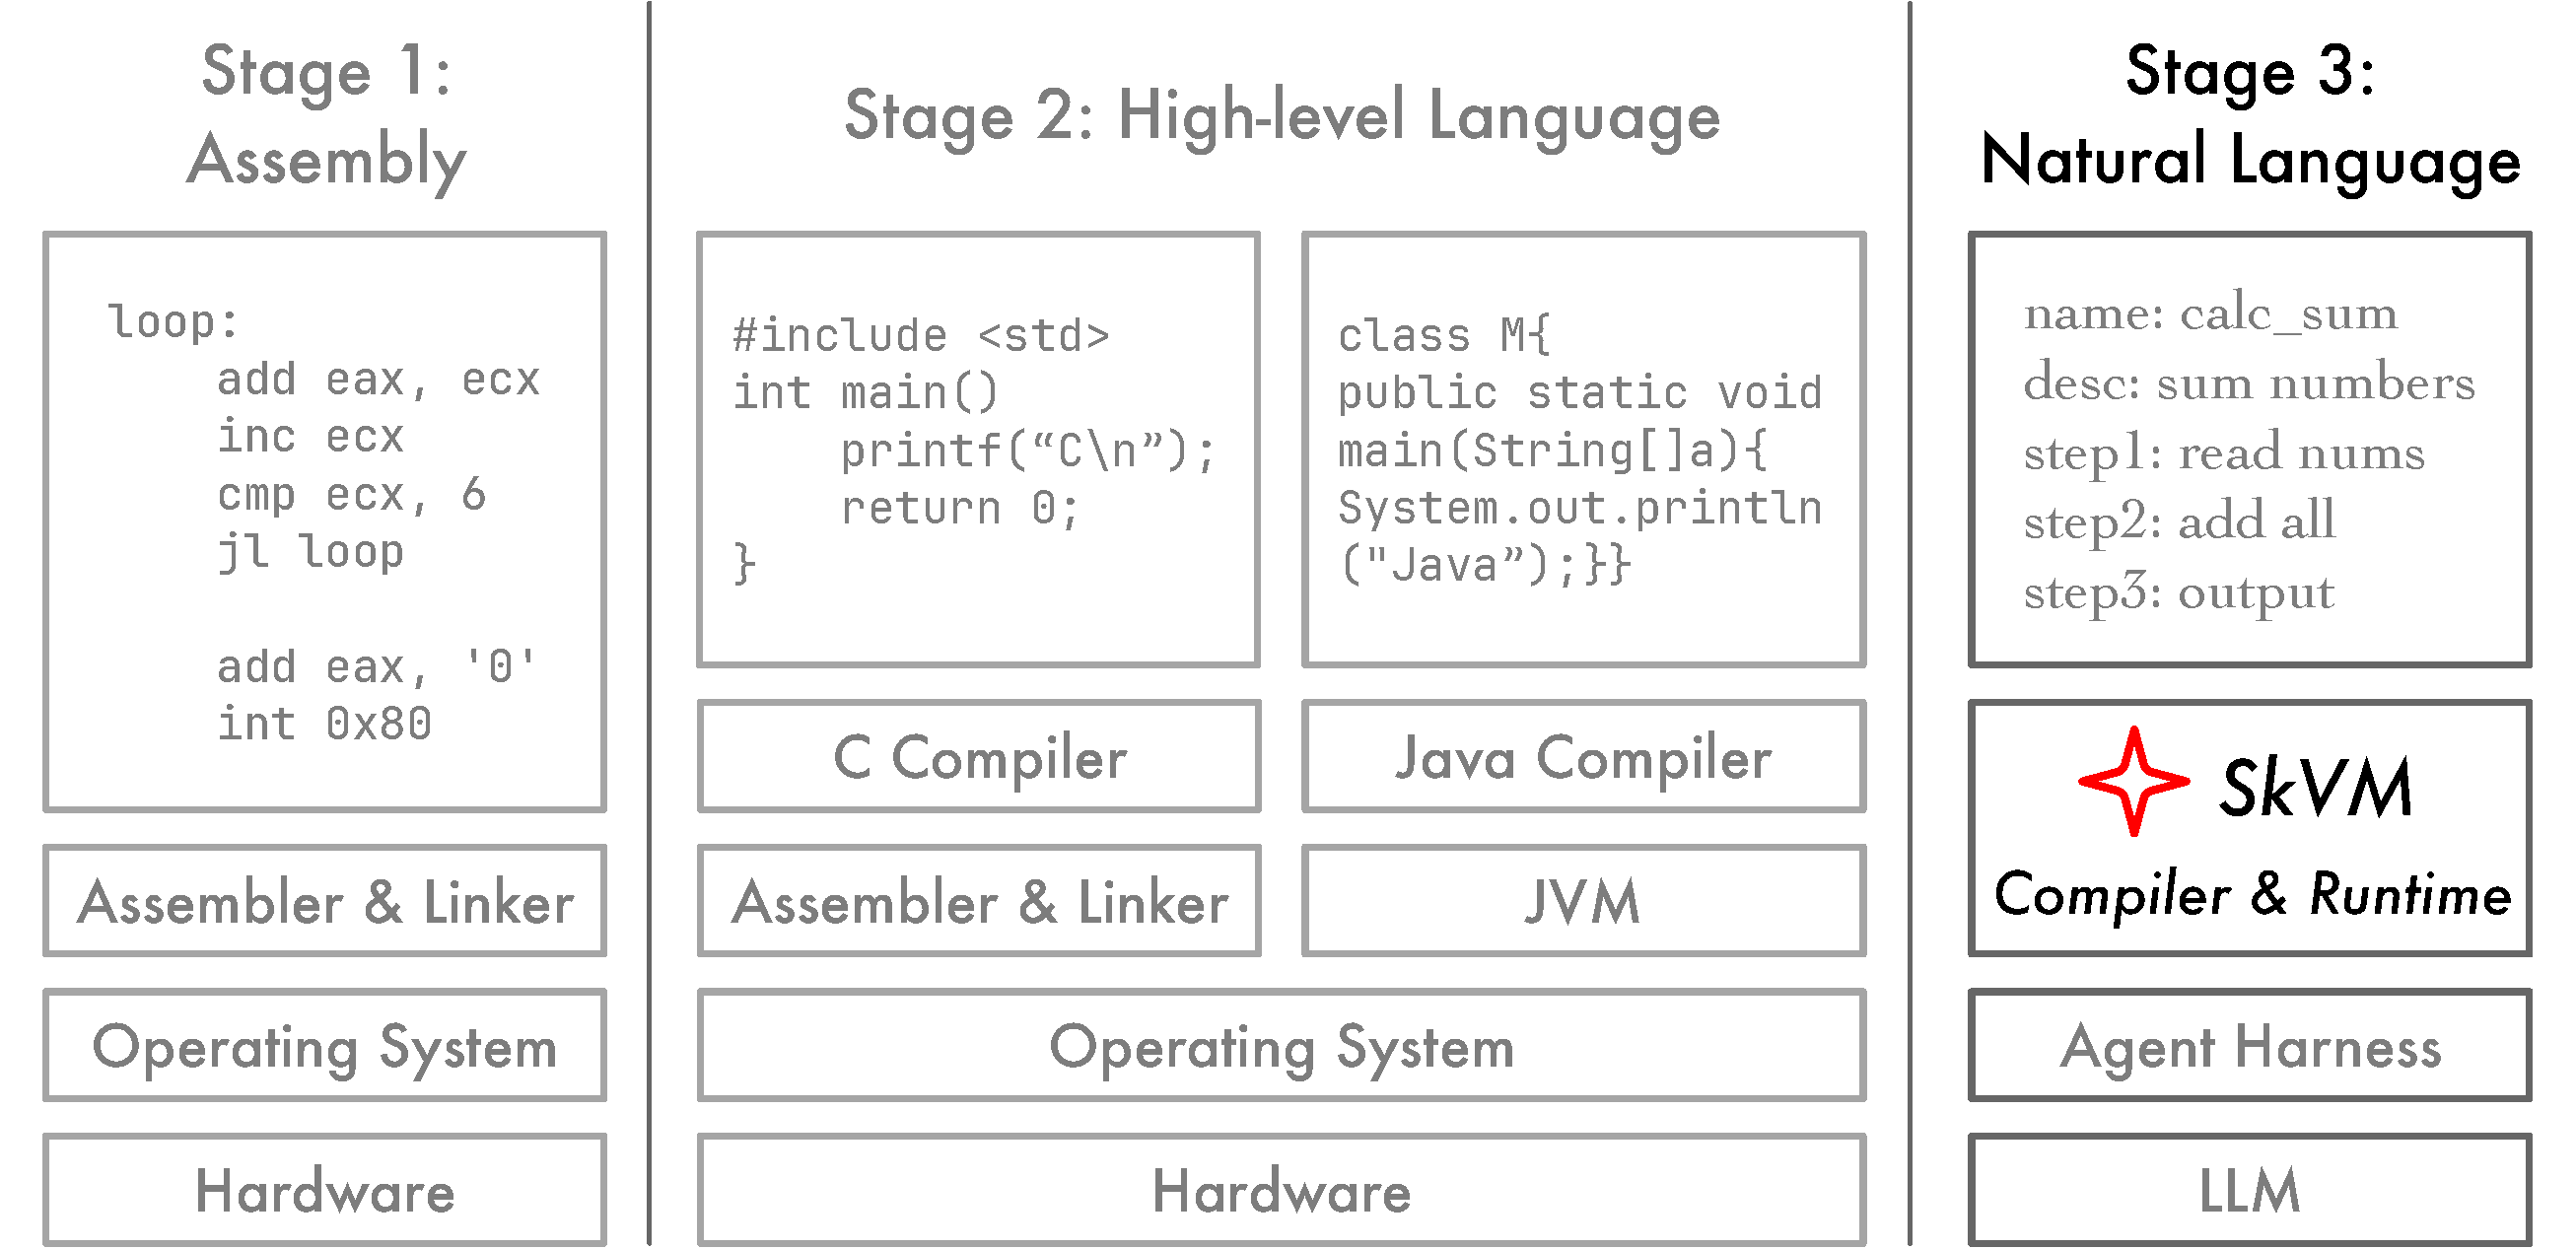
\includegraphics[width=\columnwidth]{figures/skillos_arch.pdf}
  \caption{编程抽象的演进。技能处于当前前沿：它们是长达数百行的自然语言程序，却缺少支持跨目标端可移植性的编译器与运行时。}
  \label{fig:evolution}
\end{figure}

我们将这些问题归因于两个因素：（1）即使技能已被加载，模型在执行期间也可能忽略其指导；
（2）即使模型遵循技能，技能对模型能力的假设也可能与模型的实际水平不符。
除了任务完成增益上的差异，当前技能中常见的半结构化代码片段和工作流式格式
还会产生大量 token 开销（例如 token 增加 451\%，而通过率保持不变~\cite{han2026swe}）并带来更高的执行延迟。

这一问题源于静态技能与底层模型及代理框架的多样性之间存在根本错配。
技能所要求的能力可能与运行时调用的 LLM 所具备的能力不一致。回顾计算范式的演进~\cite{stroustrup2013c++, venners1998java, cramer1997compiling}（如图~\ref{fig:evolution} 所示），我们观察到：
在代理时代，\textbf{技能就是代码}，而\textbf{LLM 就是处理器}。但目前并不存在一种机制，
能够让技能在异构 LLM 与代理框架之间得到高效且可靠的执行。

受到经典计算系统处理代码方式的启发，我们提出
\sys，一个面向技能的编译与运行时系统；它支持
高效的跨模型执行，并为技能执行提供统一的底层支持。
借助 \sys，技能会被编译为针对不同模型定制的形式，使每个模型都能
更好地理解和执行技能。此外，\sys 提供统一的运行时
环境，对技能加载、解析与并发执行进行系统化管理。

\textit{我们围绕经典编译技术来组织 \sys：
解释执行~\cite{jansen2007interpretation}、提前（AOT）编译~\cite{serrano2021javascript, serrano2018javascript}，以及即时（JIT）
优化~\cite{aho2006compilers, aycock2003jit, suganuma2000overview, ishizaki2000study, cramer1997compiling}。}
目前，代理只使用解释执行来处理技能，即把原始技能文本直接送入模型。
这种方法妨碍了技能的可移植性与执行效率。相比之下，\sys 进一步采用
AOT 和 JIT 编译，针对不同的后端模型与执行环境进行优化：

\textbf{AOT 编译：}技能内在地编码了对模型能力、环境配置和并行机会的需求。
因此，\sys 会在执行前分析这些需求并据此优化技能。
\emph{基于能力的编译}提取 26 项原语能力，用它们刻画 LLM 与技能需求之间的能力缺口。
每项能力以多个熟练度等级抽象模型行为的一个独立维度。
编译器沿这些能力维度测量目标模型，并调整技能规范，使之更好地适配模型的优势与局限。
其次，\emph{环境绑定}从技能描述中提取对软件包和工具的隐式依赖，并生成可在加载时执行的设置脚本，保证技能执行前所有依赖均已满足。
最后，\emph{并发性提取}借鉴经典编译器对数据级并行（DLP）~\cite{kalathingal2016dynamic}、指令级并行（ILP）~\cite{ranganathan1998empirical, kastner2001ilp} 和线程级并行（TLP）~\cite{redstone2003mini} 的优化方法，从技能中提取相应的三种粒度的并行机会，并将其显式暴露给代理框架，从而提高任务执行效率。

\textbf{JIT 优化：}在运行时，\sys 利用运行信息持续优化技能的性能与正确性。
\emph{代码固化：}技能可能包含参数化脚本模板，这些模板会在不同执行中被多次实例化。
JIT 编译把这些高频模板具体化为已实例化的可执行代码，从而绕过 LLM 解析。
\emph{自适应重编译：}JIT 监控会跟踪模型执行，并在出现能力缺口时自适应地重编译技能，
使技能能够通过迭代优化实现自我改进。

技能编译完成后，技能运行时解析的是编译后的技能产物（包括优化后的
技能、已实例化脚本和并发依赖图），而非简单地把原始文本传给模型。
此外，技能运行时还会结合系统可用资源与工具能力，
实时调度代理执行，保障执行过程稳定可靠。

我们在规模各异的八个 LLM 与三个代理框架上评估 \sys，覆盖 SkillsBench~\cite{li2026skillsbench} 和具有代表性的技能任务（共 118 个任务）。
结果表明，\sys 在不同模型与代理框架~\cite{claudecode,opencode} 上显著提高任务完成率，平均提升 15.3\%。
此外，对于能够完成的任务，\sys 最多可减少 40\% 的 token 消耗。
在性能方面，\sys 通过细粒度并行化和 JIT 代码固化取得 3.2$\times$--50$\times$ 的端到端时间加速。
